\chapter{Importing and exporting}
\label{txt:importExport}
Importing and exporting of dendro data in Tellervo is provided through the TRiCYCLE libraries.  TRiCYCLE is a universal dendro data conversion application for converting back and forth between 24 supported data formats \citep{tricycle}.  The open source libraries that provide the functionality to TRiCYCLE are incorporated directly into Tellervo providing support for all these formats.  

\begin{table*}[htbp]
\centering
\label{txt:formatList}
\index{File formats}
\begin{tabular*}{0.8\textwidth}{ll}
\toprule
Belfast Apple & Nottingham \\
Belfast Archive & ODF Spreadsheet \\
Besancon (including SYLPHE variants) &   Oxford\\
CATRAS & PAST4\\
Cracow Binary Format & Sheffield D-Format (Dendro for Windows)\\
Comma delimited text files (CSV) &  Topham \\
Corina Legacy &  TRiDaS\\
DendroDB & TRIMS\\
Heidelberg (TSAP-Win) &  Tucson (RWL and CRN)\\
KINSYS-KS & Tucson Compact\\
Microsoft Excel 97/2000/XP & VFormat \\
Microsoft Excel 2007 & WinDENDRO\\
\bottomrule
\end{tabular*}
\caption{List of the twenty-four formats supported by Tellervo. See appendices \ref{txt:fileFormatsStart}--\ref{txt:fileFormatsLast} (pages \pageref{txt:fileFormatsStart}--\pageref{txt:fileFormatsEnd}) for full descriptions.}
\end{table*}



\section{Exporting data}
\index{Export!Data}
Exporting data is initiated by the \menutwo{File}{Export data menu}.  If this is called from the main Tellervo data window, it will export the current series.  If it is called from the Tellervo home screen, then it will present you with the database browser and allow you to pick one or more series to export.  If you use the menu from within the main data editor then it will export 

\begin{SCfigure}
  \centering
    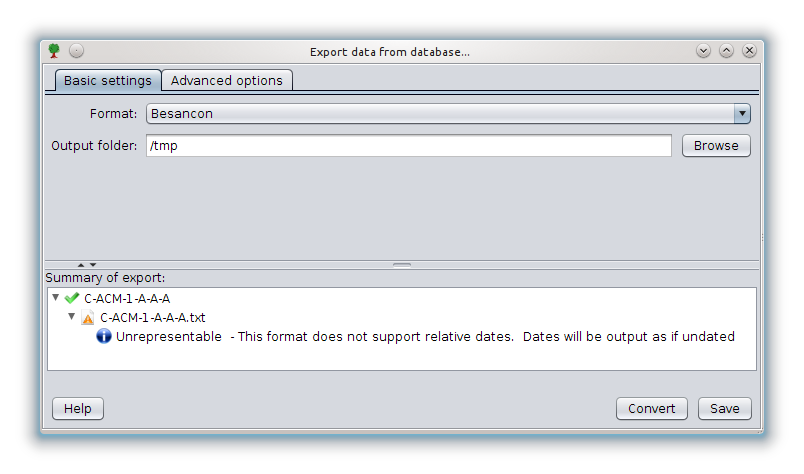
\includegraphics[width=0.7\textwidth]{Images/exportdata1.png}
    \caption{Screen showing a series that has been exported to Besan\c{c}on format.  In the summary of the export at the bottom of the screen you can see the warning to the user that this format does not have the ability to represent relative dates properly.}
    \label{fig:exportdata}
\end{SCfigure}

The export dialog contains two tabs.  The first allows the user to choose the format that they would like to export to and the folder into which to save the result.  Note that the user needs to specify a folder not a filename as many formats are unable to store more than one series in a file.  When exporting derived series such as chronologies, the export dialog may therefore need to create multiple files.  The second tab contains advanced options for altering the behaviour of the exporter:

\begin{description}
 \item[What to export] -- This option enables the user to choose between exporting just the current series, or the current series and all associated series
 \item[Grouping]  -- This enables the user to choose to group files into a single export file if possible.  For formats that do not support more than one series in a file, this option is ignored.
 \item[Naming] -- This configures how the output files are named.  See section \ref{txt:namingConventions} for more details.
 \item[Encoding] -- This specified the character encoding to use in the exported text file. See section \ref{txt:characterSets} for more information. 
\end{description}

\subsection{Naming conventions}
\label{txt:namingConventions}
\index{Naming conventions}
The naming convention is used to determine how to name the output files. The naming convention
relates to the filename itself and not the file extension. The file extension is specific to the output format
chosen (e.g. Heidelberg files are .fh and TRiDaS files are .xml).

\begin{description}
 \item[Numerical] -- This is the default naming convention. It uses the name of the input data file and
appends an incrementing number if more than one output file is produced.
 \item[UUID] -- This gives all output files a random named based on Universally Unique Identifiers
(UUIDs). This is a 36 character hexadecimal code which due to the astronomically
large number of possible combinations is guaranteed to be universally unique. A
typical filename will look like: 550e8400-e29b-41d4-a716-446655440000.
 \item[Hierarchical] -- This uses the hierarchical structure of the TRiDaS data model to provide a meaningful
name for the output file. It joins together the title of each entity in the file beginning
with the project name through to the series name. For files that contain multiple series,
the name will contain details of all the entities shared by all the series in the file. For
example, if a file contains several series from the same sample, then the file name
will be projectTitle-objectTitle-elementTitle-sampleTitle. If the file contains several
series from different samples of the same object, then the file would be projectTitle-
objectTitle. If multiple output files end up with the same name then like the numerical
convention described above, the files will have an incremental number appended to
the end. Unfortunately, most input data files do not contain rich name information
so files end up being called unnamedProject-unnamedObject-unnamedElement etc.
This convention is therefore more appropriate when converting from TRiDaS to other
formats.
\item[Series code] -- This convention is only applicable to formats that contain just one series.  The file is named according to the series code.
\item[Series code (8 characters)] -- Same as `Series code', however the file name is truncated to 8 characters if the series code is longer.  
\item[Keycode] -- Similar to `Series code' but preferentially uses a keycode (supplied by some file formats) if available.  If a keycode is not provided, then it falls back to using the series code.
 \end{description}

Note that some formats (e.g. CATRAS) require the file name to be the same as a field within the file.  In this case the naming convention is overidden, so no matter what convention you specify the filename will be the same.  If you manually rename a CATRAS file you will come across errors when loading it in the CATRAS application.

\subsection{Character sets}
\label{txt:characterSets}
\index{Character sets}
\index{Encoding}
Character sets are the
mechanism for pairing computer character codes with the character glyphs that we read. The widely
used standard was originally ASCII, but this does not include diacritic characters, and characters specific
to certain languages. There have since been many character encodings proposed (e.g ISO 8859-1 for
Western Europe and ISO 8859-7 for Greece) as well as some that are specific to Windows and Mac
operating systems (e.g. Windows-1252 and MacRoman). The character set that is becoming most widely
used today is Unicode UTF-8. This is capable of representing the vast majority of characters (107,000+) while remaining
backwards compatible for the 128 characters that ASCII is able to represent.

If an incorrect character encoding is used to interpret a file, normally the majority of characters will display
correctly (where the character sets share the same encodings) but more unusual characters will be displayed
incorrectly - typically square boxes or question marks.

The character encoding is set to the default for the operating system you are running. For instance on
MacOSX this will be MacRoman and for Windows it will be Windows-1250. If you know your input file
is in a different encoding you should set it in the input charset box. If your output file needs to be read
on an operating system other than the one you are currently running, then you may like to override the
writer charset. Please note that for certain writers, the character set used is part of the file specification
(e.g. TRiDaS must be UTF-8). In this case your choice will be ignored.

The final complication with regards character sets is the line feed character(s). For historical reasons
different operating systems use different characters to represent a new line. Depending on the software
that is used to read a file, this can cause problems. Tellervo itself will automatically adapt to files with
any type of line feed characters so reading files in Tellervo will never be a problem. When writing
out files, Tellervo will use the default line feed for the operating system you are running, unless you
choose a platform specific character set. For instance if you run Tellervo on Windows and choose a
MacRoman writing charset, Tellervo will use Mac style line feeds.

\section{Importing data}
\index{Import}

Although the TRiCYCLE import library can easily read the data from many data files, the process of importing files is complicated by the need to cross-map which sites, trees etc the data corresponds to and whether they are already in the database or not.  

\begin{figure}[hbtp]
  \centering
    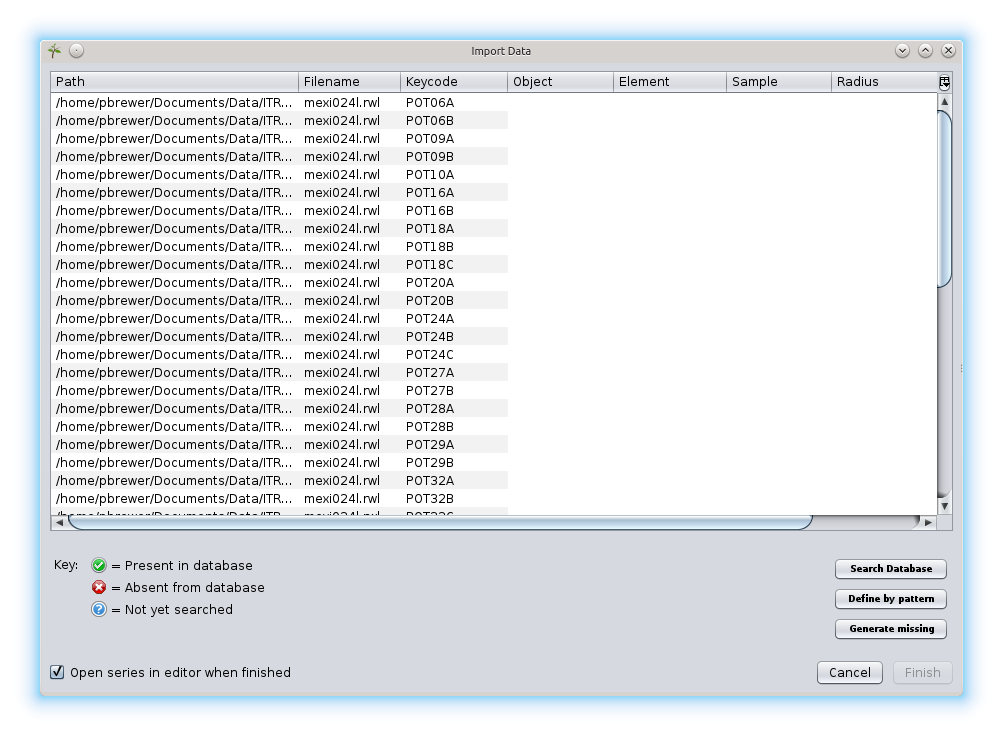
\includegraphics[width=\textwidth]{Images/dataimport.png}
    \caption{The data import dialog is used to assign data from legacy data files to the correct entries in the Tellervo database.}
    \label{fig:dataimport}
\end{figure}

The data import process is accessed via the \menutwo{File}{Import data} menu.  Choose the file format that you would like to import, then select on or more files.   If you are unsure what format your file is in, you can use appendices \ref{txt:fileFormatsStart}--\ref{txt:fileFormatsLast} (pages \pageref{txt:fileFormatsStart}--\pageref{txt:fileFormatsEnd}) to help you.  You may also like to download TRiCYCLE\footnote{TRiCYCLE is available from \url{http://www.tridas.org/tricycle}} which includes a file identification tool in the help menu.

\warn{The Tellervo system is currently limited to reading in raw data files.  It does not allow for reading in of chronology files as these contain a more complex level of metadata.  Support for chronology files will be included in a later release.}

The Import Data dialog (figure \ref{fig:dataimport}) provides a spreadsheet-like interface to assign which object, element, sample and radius in the database each imported data series should be assigned to.  It is possible to simply type the code for each of these entities into the table but for more than a few series this quickly becomes tedious.  Instead, you can automatically populate this table by defining patterns based on the file names, folder names and/or rudimentary metadata from the files.  If your data files follow a rigid naming convention this can dramatically speed up the import process.  To use this feature click the `define by pattern' button to show the define patterns dialog (figure \ref{fig:importdatapatterns}).

\begin{figure}[hbtp]
  \centering
    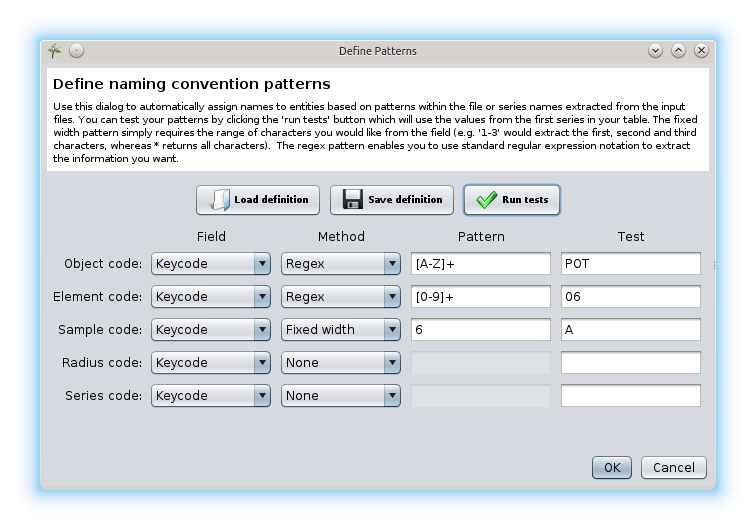
\includegraphics[width=\textwidth]{Images/importdatapatterns.png}
    \caption{Data patterns dialog used to define naming conventions to automate the mapping of legacy data to entries in the Tellervo database.  The example here is for a series with a keycode of `POT06A'.  The first regular expression extracts all upper case alphabetical letters at the start of the keycode for the object code.  The second regular expression extracts the digits for the element code.  The fixed width pattern extracts the 6 character for the sample code.}
    \label{fig:importdatapatterns}
\end{figure}

For each of the object, element, sample, radius and series codes, you can define patterns for mapping your data to the database.  These codes may be based in whole or in part on: file name; full folder path; final folder; and keycode extracted from the file.  You can specify a variety of methods for extracting information from these fields:

\begin{description}
\item[All] -- This simply takes the entire field you specify.  For example if the data file was called abc.rwl and you asked for `all' of the filename field, then you would get abc.rwl
\item[Fixed width] -- This allows you to specify a fixed number of characters specified either as an absolute number or a range.  For example, if you were to specify  1-3 for the filename abc.rwl, then you would get abc.  This is a simple method but relies on your data files all following the same convention and with the same number of characters.
\item[Regex] -- This is a far more powerful method, but more complicated to master.  Regex stands for regular expression and is an advanced language for defining patterns.  A full description of the syntax is beyond the scope of this manual but there are many resources on the Internet to help.   
\end{description}

Once you have set your method and pattern you can press the `run tests' button to check your pattern matches what you expect.  The test field will show the result of running the first series in your import through your pattern.  If the results aren't as you expect you can modify your pattern and re-run the tests.  The dialog also has the ability to load and save your pattern definitions.  This is particularly helpful if you are lucky enough to have many data files that match a specific naming convention.

Once you are satisfied with your patterns you can click OK to return to the data import screen.  The fields in the table will be populated with the matches as defined by your patterns with the entries marked by one of three icons.  These denote whether a record with this code exists in the database, whether it is currently absent from the database, or whether the database has not yet been searched.  Clicking the `search database' will check the database for all unsearched records turning them from a blue question mark to a red cross or green tick accordingly.  

Once you are satisfied that all entries in the table are correct you can go ahead and press the `generate missing' button to create entries in the database for each record currently marked with a red cross, turning them green.  Once the table is full of green ticks, the `finish' button will become enabled.  If the `open series in editor when finished' tickbox is checked, then all these series will be opened in the main window. If your file does not explicity indicate what units the measurements are in, a dialog box will ask you to specify.  

Please note that all the newly generated database entries will be skeleton records.  You will need to check and update the metadata for each of these to ensure they fulfill the requirements of Tellervo.  For example, many mandatory Tellervo fields are missing from legacy data files.  Even fields that are present (such as taxon) are typically not standardised well enough to match the specific controlled vocabularies used in Tellervo.



